\documentclass[11pt]{article}
\usepackage[T1]{fontenc}
\usepackage[utf8]{inputenc}
\usepackage{amssymb}
\usepackage{amsmath}
\usepackage{tikz}
\usetikzlibrary{arrows,fit,positioning,calc}
\usepackage{pgfplots}
\pgfplotsset{width=7.5cm,compat=1.16}
\pgfdeclareshape{document}{
\inheritsavedanchors[from=rectangle] % this is nearly a rectangle
\inheritanchorborder[from=rectangle]
\inheritanchor[from=rectangle]{center}
\inheritanchor[from=rectangle]{north}
\inheritanchor[from=rectangle]{south}
\inheritanchor[from=rectangle]{west}
\inheritanchor[from=rectangle]{east}
% ... and possibly more
\backgroundpath{% this is new
% store lower right in xa/ya and upper right in xb/yb
\southwest \pgf@xa=\pgf@x \pgf@ya=\pgf@y
\northeast \pgf@xb=\pgf@x \pgf@yb=\pgf@y
% compute corner of ‘‘flipped page’’
\pgf@xc=\pgf@xb \advance\pgf@xc by-10pt % this should be a parameter
\pgf@yc=\pgf@yb \advance\pgf@yc by-10pt
% construct main path
\pgfpathmoveto{\pgfpoint{\pgf@xa}{\pgf@ya}}
\pgfpathlineto{\pgfpoint{\pgf@xa}{\pgf@yb}}
\pgfpathlineto{\pgfpoint{\pgf@xc}{\pgf@yb}}
\pgfpathlineto{\pgfpoint{\pgf@xb}{\pgf@yc}}
\pgfpathlineto{\pgfpoint{\pgf@xb}{\pgf@ya}}
\pgfpathclose
% add little corner
\pgfpathmoveto{\pgfpoint{\pgf@xc}{\pgf@yb}}
\pgfpathlineto{\pgfpoint{\pgf@xc}{\pgf@yc}}
\pgfpathlineto{\pgfpoint{\pgf@xb}{\pgf@yc}}
\pgfpathlineto{\pgfpoint{\pgf@xc}{\pgf@yc}}
}
}

\begin{document}

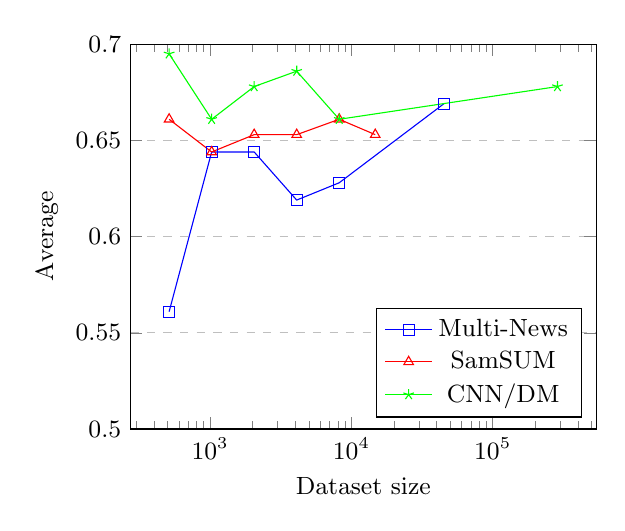
\begin{tikzpicture}
\centering
\small
\begin{axis}[
    title={},
    xlabel={Dataset size},
    ylabel={Average},
    ymin=.5, ymax=.7,
    legend pos=south east,
    ymajorgrids=true,
    grid style=dashed,
    xmode=log,
]

\addplot[
    color=blue,
    mark=square,
    ]
    coordinates {
    (512,.561)(1024,.644)(2048,.644)(4096,.619)(8192,.628)(44972,.669)
    };
    
\addplot[
    color=red,
    mark=triangle,
    ]
    coordinates {
    (512,.661)(1024,.644)(2048,.653)(4096,.653)(8192,.661)(14732,.653)
    };

 \addplot[
    color=green,
    mark=star,
    ]
    coordinates {
    (512,.695)(1024,.661)(2048,.678)(4096,.686)(8192,.661)(287113,.678)
    };
    \legend{Multi-News,SamSUM,CNN/DM}
 
    
\end{axis}
\end{tikzpicture}

\end{document}